\chapter{State of the Art}\label{chap:stateOfTheArt}

\begin{mybox}
This chapter is dedicated to the introduction of the basic notions of this thesis.
Concretely speaking, we are going to present the state of the art constituting of mainly three basic contents:

\begin{itemize}
    \item Several modeling frameworks, some of which are the ancestors of the new modelings to be used in this thesis and some of which will be used in comparison
    \item The notion of model-checking and some existed model checkers 
    \item Different update schemes of modeling frameworks
    \item Several model learning/inference techniques
\end{itemize}

These notions will be helpful for readers to understand our new model-checkers and new model inference approaches.
\end{mybox}

In computational biology, there are plenty of modeling frameworks suiting different needs.
Model is a useful tool to represent the abstraction of the real system, as the real system is usually mechanically complicated and not completely known.

From the point of view of data type, models are classified into continuous ones, discrete ones and their combination, hybrid models, where the last one is not the focus of this thesis.

Continuous models are usually derived from real world data, as the data (no matter time-series data or static data) are obtained by measurement and can be used as input without preconditioning.
Differential equations models~\cite{glass1973logical,snoussi1989qualitative,thomas1990biological} are based on the hypothesis that in biological systems, the change rate of variables is numerically related to the values of other variables. 
Differential equations models deal with mainly the system dynamics, \textit{i.e.} biological regulations.
Models based on Bayesian probability and Markov chain~\cite{huelsenbeck2001mrbayes,larget1999markov} study static topics, \textit{i.e.} phylogenetics.

However, the following difficulties usually arise in the analysis of continuous models:

\begin{itemize}
    \item System mechanics is unclear
    \item System parameters need to be precise which is difficult for biological system
    \item Solving differential equations numerically is expensive 
\end{itemize}

Unlike straightforward continuous modelings, discrete modelings perform an abstraction of continuous dynamics and an over-approximation of continuous constraints~\cite{bernot2009}.
Discrete models can be also inferred from discrete data by discretization~\cite{dimitrova2006polynomial}.

On the aspect of dynamics, discrete models have the following update pattern: $discrete\_state1\xrightarrow{conditions}discrete\_state2$, where the states correspond to the intervals in the continuous models. 
States here can be qualitative levels or \textit{combination}s of qualitative levels, compensating the imprecision or the incompleteness of the original system.
Conditions here could be either a necessary time delay or a state of the current system, \textit{etc}.

As to the computation of various properties, discrete transition models generally cost less than continuous dynamical models.
Among discrete models, Boolean Networks~\cite{kauffman1969}, Thomas Models~\cite{thomas1978}, Petri nets~\cite{pinney2003petri}, Process Hitting Framework~\cite{pauleve2011} could more or less avoid these disadvantages when facing the problems related to system evolution.

Hybrid (in the sense of discrete/continuous) models~\cite{wang2015sreach,lincoln2004symbolic,singhania2011hybrid} usually behave like continuous models, because in each discrete block, the sub-model also need continuous parameters as continuous models need.
Their computational complexities are of the same scale.
We are not going to detail hybrid models during this thesis.

Continuity characterizes the evolution pattern of each variable.
However, models contain multiple variables.
From the point of view on concurrency, models can be classified according to update schemes into mainly three genres: synchronous models, asynchronous models and generalized models.

Synchronous update scheme designates that every component will transit simultaneously to one of its possible future states regardless the time needed for transition or other components.
However in real world, constraints always exist.
Biologically it is not probable that multiple components in one system change their state simultaneously.
This deficiency demands us to consider more update schemes.
Detailed discussion is in Section~\ref{sec:semantics}.

In this chapter, we will first discuss several discrete modeling frameworks and updating schemes, comparing their differences and the possibility of translating from each other.
Some of these models will be used in the following chapters.
Models need related analytic tools, we will then study some model checkers especially those focusing on reachability properties as many other complex properties can be formulated with the help of reachability.
At last we will be interested in the model learning and revising techniques which are the key of constructing a model.

\section{Discrete Modeling Frameworks}
Original biological problems are usually difficult to be studied directly due to the uncertainty and the big scale of biological systems. 
Modeling is a process of abstracting the real system into a more concise and more easily automatized system.
To solve a certain problem, an appropriate modeling framework is crucial because different models have different bias from reality and have also different advantages in computation, e.g. fixed point, reachability etc.
Here we are going to introduce several most frequenly applied modeling frameworks and analyze their advantages and disadvantages.

\subsection{Regulatory Network}\label{sec:regNetwork}
Regulatory Networks (RN) have characteristics of a static network, representing the interactions between components~\cite{bernot2009}.
With the analysis of topological features, it can be applied in for example gene expression analysis~\cite{shinozaki2003regulatory}.

\begin{definition}[Regulatory network (RN)]\label{def:RN}
A regulatory network is a labeled digraph $G=(V,E)$ where 
\begin{itemize}
    \item each vertex $v$ of $V$, called variable, is provided with a boundary $b_v\in \mathbb{N}$ less or equal to the out-degree of v in G.
    \item each arc $u\in v$ of $E$ is labelled with a couple ($t_{uv}$, $\alpha_{uv}$) where $t_{uv}$ is an integer between 1 and $b_v$, called qualitative threshold and where $\alpha_{uv}\in \{+,-\}$ is the sign of the regulation.
\end{itemize}
\end{definition}

An example is shown in Figure~\ref{fig:booleannetwork} A, consisting of three entities $X,Y,Z$.
Sharp arrows $\to$ stand for promotion while blunt arrows $\dashv$ stand for inhibition,
\textit{e.g.} $X$ inhibits $Z$, $Z$ promotes $Y$.

RN is a special instance among discrete modelings.
It does not require a threshold setting for each variable.
As a result, RN is usually applied to study static problems, e.g. model completion, finding fixed points~\cite{yamamoto2014completing}.
Without quantitative representation, one can barely analyze the system dynamics because RN does not possess an update pattern which describes state transitions.

\subsection{Bayesian Network}
Bayesian networks are a type of probabilistic graphical models. 
They represent joint probability distribution of a set of variables.
More concretely, if one obtains the value of certain variable, a Bayesian network can help him analyze the values of its linked variables.

Bayesian networks are usually used for inferring causal dependencies between genes in gene regulatory networks with the goal of estimating the posterior probability of chosen features being inherent in the network, given the data~\cite{friedman2000using}.

A Bayesian network is defined as $(G, \theta)$ where $G$ is a \textit{directed acyclic} graph whose vertices connect the random variables of the network.
$\theta$ is a probability distribution associated to the vertices. 
These variables can be continuous or discrete. 
Directed edges correspond to dependencies between variables. 
$\theta$ describes a conditional distribution for each variable of the network, given its ``parents'' as defined by the relations in $G$.

One disadvantage of Bayesian networks is that they can only represent acyclic topology as they must be acyclic in order to guarantee that their underlying probability distribution is normalized to $1$.
However feedback loops appear very frequently in biology which narrow the application of Bayesian networks.

\subsection{Boolean Network}
Boolean Networks (BN) are a traditional framework studied for decades~\cite{kauffman1969}.
They discretize every variable of the system into Boolean variables $0$ and $1$, presenting active/inactive, high/low concentration, \textit{etc}. 
Transitions in BNs are defined by Boolean functions, here we will introduce its basic definition.

\begin{definition}[Boolean Network (BN)]
A Boolean Network $G(V,F)$ consists of a set of nodes $V=\{v_1,\cdots,v_n\}$ and a set of Boolean functions $F=\{f_1,\cdots,f_n\}$ where function $f_i$ decides the value of node $v_i$ of the next time point: $v_i(t+1)=f_i(v_1(t),\cdots,v_n(t))$.
\end{definition}



In some applications, the nodes are classified into incoming nodes, outgoing nodes and inner nodes to represent an input-output system~\cite{akutsu2007control}.

\begin{figure}[ht]
    \centering
    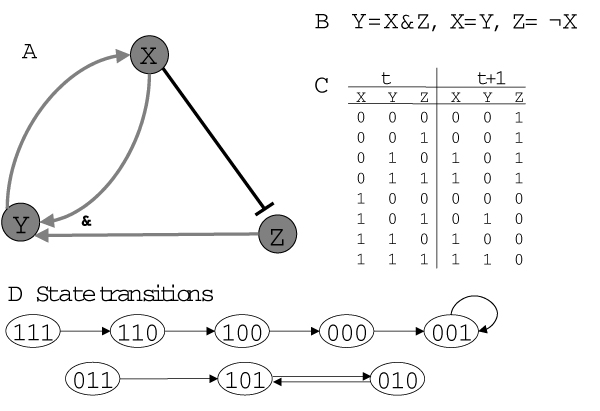
\includegraphics[width=0.7\textwidth]{BooleanNetwork.png}
    \caption[Representations of Biological Topology]{Four ways of representing biological topology: A. regulatory network, B. Boolean functions, C. transition interpretation table, D. State transition graph}
    \label{fig:booleannetwork}
\end{figure}

Figure~\ref{fig:booleannetwork} shows different representations of biological topology.
RN (A) shows only a qualitative inference graph.
BN (B) is concise but does not indicate directly the state change between moments $t$ and $t+1$.
Its update scheme needs to be precised (in Section~\ref{sec:semantics}).
Transition interpretation table (C) and state transition graph (D) are straightforward but there are two drawbacks: 
\begin{itemize}
    \item the state space increases exponentially with the number of variables leading to the lack of memory
    \item they are not equivalent to Boolean functions
\end{itemize}
One set of transition interpretations or one state transition graph could correspond to multiple set of Boolean functions.

In term of expressiveness, BNs can be translated to Normal Logic Programs (NLP)~\cite{inoue2011logic}.
NLP provides a more dynamical representation and also for applying SAT techniques in the computation of point attractors of both synchronous and asynchronous semantics~\cite{dubrova2011sat,harvey1997time}.

\subsection{Normal Logic Program (NLP)}\label{sec:logicProgram}
Logic programming is a type of programming paradigm which is largely based on formal logic.
Any program written in a logic programming language is a set of sentences in logical form, expressing facts and rules about some problem domain.
Major logic programming language families include Prolog, Answer set programming (ASP, which we will detail in Section~\ref{sec:introAsp} of Chapter~\ref{chap:refinement}) and Datalog.

In all of these languages, the basic element is called an \textit{atom}, representing a variable with certain value.
The set of atom is denoted $\mathcal{B}$.
Rules are written in the form of clauses consisting of atoms (formula representation on the left while code representation on the right):

\begin{table}[ht]
    \centering
    \begin{tabular}{ccc}
        $H \gets B_1\land\ldots\land B_n.$  & or & \texttt{H :- B1, ... , Bn.}
    \end{tabular}
\end{table}

$H,B_1,\ldots,B_n$ are atoms. 
The rule is read declaratively as logical implications:

\begin{center}
    $H$ if $B_1$ and $\ldots$ and $B_n$.
\end{center}

$H$ is called the head of rule and $B_1,\land\ldots\land B_n$ is called the body of rule.
Facts are rules having no body, and are written in the simplified form:

$$H.$$

Using this notation, one can describe the transition of variable:

    $$var_0^{val_0}(t+1) \gets var_1^{val_1}(t)\land \ldots \land var_n^{val_n}(t).$$
    
which reads variable $var_0$ will take value $val_0$ at the next time point if variable $var_1$ takes value $val_1$ and $\ldots$ and variable $var_n$ is taking value $val_n$.
In this thesis we simplify the notation as 

$$var_0^{val_0} \gets var_1^{val_1}\land \ldots \land var_n^{val_n}.$$

\begin{remark}
NLP appears to have almost the same formula as BN according to Inoue \textit{et al.}~\cite{inoue2011logic}, the only difference is $\gets$ of NLP and $=$ of BN.
However, logic OR is not allowed in NLP.
The way to represent logic OR is to use additional rules.
For example, Boolean function $Z=X\lor Y$ can be translated to the following rules: $Z^1\gets X^1$, $Z^1\gets Y^1$ and $Z^0\gets X^0\land Y^0$.
This translation may create non-equivalence and non-determinism.
\end{remark}

Detailed applications are in Section~\ref{sec:lfit} of Chapter~\ref{chap:modelInference}.

\subsection{Process Hitting (PH)}
If one wants to describes the dynamics more finely with reasonable memory use, Process Hitting (PH) framework is a good choice, which introduced by Paulev\'e \textit{et al.}~\cite{pauleve2011}.

PH is inspired by $\pi$-calculus, which expresses the communication between canals. 
In PH, the corresponding meaning becomes the interaction between different components.
Process Hitting is an asynchronous automata network, i.e. allowing at most one transition fired simultaneously. 
PH is more expressive than Asynchronous Thomas' model~\cite{thomas1978} or Asynchronous BN. 
Actions in Process Hitting are more capable of describing various transitions than Boolean functions or attractors as it specifies the regulating and regulated components and their quantitative levels.
Also it expresses explicitly the cooperation between several components and stochastic features using $\pi$-calculus which are not detailed in this report~\cite{pauleve2014}.

Moreover, in order to define efficient analysis techniques that avoid to build the whole state space of the model causing state space explosion (in Thomas' model and Boolean network), various abstract structures have been introduced, and one of them is graph of causality, which allows a reasoning of the reachability of local states instead of traverse of global states.

It gathers a finite number of concurrent processes grouped into a finite set of sorts. A process belongs to one and only one sort and is denoted as $a_i$ where $a$ is the sort and $i$ the identifier of the process within the sort $a$.
At any time, only one process of each sort is present, forming a state of the PH.

\begin{definition}[Process Hitting (PH)]
A $PH$ consists of a tuple $(\Sigma, L, H)$:
\begin{itemize}
    \item $\Sigma=\{a,b,...\}$ is the finite set of sorts
    \item $L=\prod_{a\in\Sigma}{L_a}$ is the set of states with $L_a=\{a_0,...a_{l_a}\}$ the finite and countable set of states of sort $a\in\Sigma$ and $l_a$ a positive integer with: $a\neq b\to \forall(a_i,b_j)\in L_a\times L_b,a_i\neq b_j$
    \item $H=\{h=a_i\to b_j\Rsh b_k\mid(a,b)\in\Sigma^2, (a_i,b_j,b_k)\in L_a\times L_b\times L_b,b_j\neq b_k, a=b\to a_i=b_j\}$ is the finite set of actions, which defines the regulations and dynamics of the PH: $a_i$, $b_j$, $b_k$ are denoted $hitter(h)$, $target(h)$ and $bounce(h)$ respectively of the action $h=a_i\to b_j\Rsh b_k$.
\end{itemize}
\end{definition}

\begin{example}
Figure~\ref{fig:PH} shows a PH constituting of four sorts $a$, $b$, $c$, $d$ with initial state $\init{a_1,b_0,c_0,d_1}$. 
It has actions $H=\{\acmph{a_0}{c_0}{c_1},\ \acmph{a_1}{b_1}{b_0},\ \acmph{c_1}{b_0}{b_1},\ \acmph{b_1}{a_0}{a_1},\ \acmph{b_0}{d_0}{d_1},\ \acmph{d_1}{b_0}{b_2},\ \acmph{c_1}{d_1}{d_0}\}$. 
e.g. \acph{a_0}{c_0}{c_1} means if sort $a$ is at level 0, it allows sort $c$ to jump from level 0 to level 1.
\end{example}

\begin{figure}[ht]
\centering
\begin{tikzpicture}%[font=\scriptsize]
%\path[use as bounding box] (0,-1) rectangle (4,4);
%{left, right, top, bottom}
\TSort{(0,0)}{a}{2}{l}
\TSort{(3,0)}{b}{3}{l}
\TSort{(6,0)}{d}{3}{r}
\TSort{(2,-2)}{c}{2}{b}
\THit{a_1}{}{b_1}{.west}{b_0}
\THit{a_0}{}{c_0}{.north}{c_1}
\THit{b_1}{}{a_0}{.east}{a_1}
\THit{c_1}{out=120,in=255}{b_0}{.west}{b_1}
\THit{b_0}{}{d_0}{.west}{d_1}
\THit{b_1}{}{d_1}{.west}{d_2}
\THit{b_2}{distance=120pt,out=30,in=40}{d_0}{.east}{d_2}
\THit{d_1}{}{b_0}{.north east}{b_2}
\THit{c_1}{bend right=80pt,distance=80pt}{d_1}{.east}{d_0}

\path[bounce,bend right]
\TBounce{b_1}{}{b_0}{.north}
\TBounce{a_0}{}{a_1}{.south}
\TBounce{d_0}{bend right=50pt,distance=40pt}{d_2}{.south}
\TBounce{b_0}{}{b_2}{.south}
;
\path[bounce,bend left]
\TBounce{d_0}{}{d_1}{.south}
\TBounce{b_0}{}{b_1}{.south}
\TBounce{c_0}{}{c_1}{.west}
\TBounce{d_1}{}{d_2}{.south}
\TBounce{d_1}{}{d_0}{.north}
;
\path[bounce,bend left]
;
\TState{a_1,b_0,c_0,d_1}
\end{tikzpicture}
\caption[Process Hitting]{Gray circles represent the initial state of sorts.
Full arrows are regulations while the following dashed arrows are the actions under the condition of certain regulation.}\label{fig:PH}
\end{figure}

Nevertheless, PH cannot encode equivalently the conjunctions in Boolean functions like $f(a)=b\land c$.

To overcome this drawback, it is needed to introduce a cooperative sort $bc$ to represent the conjunction of $b$ and $c$, with 8 actions $b_0\to bc_{10}\Rsh bc_{00}$, $b_0\to bc_{11}\Rsh bc_{01}$, $b_1\to bc_{00}\Rsh bc_{10}$, $b_1\to bc_{01}\Rsh bc_{11}$, $c_0\to bc_{01}\Rsh bc_{00}$, $c_0\to bc_{11}\Rsh bc_{10}$, $c_1\to bc_{00}\Rsh bc_{01}$, $c_0\to bc_{10}\Rsh bc_{11}$.

However, the size of this representation grows exponentially with the size of the conjunction and the behavior of cooperative sorts are not equivalent to that of BN. 
Also, this encoding introduces extra reactions, producing a temporal shift between the presence of the reactants and the playability of the reaction.

\subsection{Asynchronous Automata Network (AAN)}\label{sec:AAN}
Facing the drawback of PH, i.e. only cooperative sorts can encode reactions with conjunctions in the \textit{hitters}, Asynchronous Automata Network (AAN) is introduced by Folschette \textit{et al.}~\cite{folschette2015}.
AAN allows one to naturally model cooperations by defining several requisites for a transition.
Moreover, such automata networks are still compatible with the notion of priority, that can also be used to model different reaction rates in the model.
AAN (and, a fortiori, their restriction, the PH framework) can be considered as a subset of Communicating Finite State Machines or safe Petri Nets~\cite{pauleve2012process}.

Basically the main differences between PH and AAN are listed below. 
Sorts in PH are called automata in AAN.
Also, the definition of $H$ becomes

\begin{itemize}
    \item $H=\{A\to b_j\Rsh b_k\mid b\in \Sigma \land (b_j,b_k)\in L_b\times L_b\land b_j\neq b_k\land \forall a \in \Sigma,\ |A\cap L_a|\leq 1 \land A\cap L_b=\varnothing\}$ is the finite set of actions, which defines the regulations and dynamics of the AAN: $A$, $b_j$, $b_k$ are denoted $hitter(h)$, $target(h)$ and $bounce(h)$ respectively of the action $h=A\to b_j\Rsh b_k$.
\end{itemize}

With the new definition of $H$, we can now define actions needing multiple local states as condition.

In Chapter~\ref{chap:refinement}, we will make use of the definition of AAN by limiting the variables from multi-value ones to Boolean ones in order to obtain some interesting properties in the forthcoming reachability analysis.


\section{Semantics of Modelings}\label{sec:semantics}
For a given modeling framework, even if the components and transitions are defined, the dynamics of the system is not unique. 
Different update schemes lead to different dynamics.
The main difference lies on the relations of the number of transitions \textit{can} be fired and the number of transitions \textit{will} be fired at given time point $t$~\cite{ribeiro2018learning,chatain2018boolean}.

%\cite{ribeiro2018learning}


\subsection{Synchronicity}
Literally, synchronous update scheme implies that every fireable transition is fired simultaneously.

\begin{table}[ht]
    \centering
    \begin{tabular}{cc|cc}
        \multicolumn{2}{c|}{$t$}&\multicolumn{2}{c}{$t+1$}\\
        \hline
        $u$ & $v$ & $u$ & $v$ \\
        \hline
        0 & 0 & 2 & 0 \\
        1 & 0 & 2 & 1 \\
        2 & 0 & 2 & 1 \\
        0 & 1 & 0 & 0 \\
        1 & 1 & 0 & 1 \\
        2 & 1 & 2 & 1 \\
    \end{tabular}
    \caption{Exemplary transition interpretation table}
    \label{tab:transTable}
\end{table}


\begin{example}
Taking the transition interpretation table in Table~\ref{tab:transTable} as the given system dynamics, Figure~\ref{fig:updateScheme} (a) shows the synchronous case. 
\end{example}


Synchronous update scheme seems to be deterministic. 
However, when there are multiple fireable transition for one variable, there are multiple possible future states which cannot be fired simultaneously. 

\begin{example}\label{example:counterSynchronous}
Given an NLP with rules $var_3^1\gets var_1^1$ and $var_3^2 \gets var_2^1$
%$c_1\gets a_1$ and $c_2\gets b_1$ 
and initial state $\init{var_1^1, var_2^1, var_3^0}$,
%$\init{a_1,b_1,c_0}$
these two rules are in conflict.
Even though the semantics is synchronous, a choice is need to be made between these transitions.
\end{example}

To avoid the conflicts in Example~\ref{example:counterSynchronous}, one possible solution in Boolean NLP is to clarify the state transition metrics:
for one variable, if it can change its value at the next time point, it cannot keep its current value.

On the computational aspect, one of the benefits of the synchronous model is tractability, while classical state space exploration algorithms fail if there are multiple possible future states at each state transition.


\begin{figure}[ht]
%\begin{minipage}[ht]{0.32\textwidth}
\subfigure[0.31\textwidth][Synchronous semantics]{
\begin{tikzpicture}[scale=0.87,line width=1pt]
\draw[->] (0,0) -- (3.5,0);
\draw	[->] (0,0) -- (0,2.5);
\draw[step=1] (0,0) grid (3,2);
\node at (3.5,0)[anchor=north]{\small u};
\node at (0,2.5)[anchor=east]{\small v};
\foreach \x in {0,1,2}
\node at ($(\x,0)+(0.5,0)$)[anchor=north] {\small $\x$};
\foreach \y in {0,1}
\node at ($(0,\y)+(0,0.5)$)[anchor=east] {\small $\y$};
%\node at (1,0)[anchor=north]{$t_{uv}$};
%\node at (2,0)[anchor=north]{$t_{uu}$};
%\node at (0,1)[anchor=east]{$t_{vu}$};
\draw[->] (0.5,1.4) -- (0.5,0.6);
\draw[->] (1.4,1.5) -- (0.6,1.5);
%\draw[dotted,->] (0.6,0.5) -- (2.4,0.5);
\draw[->] (0.6,0.5) -- (2.4,0.5);
%\draw[dashed,->] (1.6,0.6) -- (2.3,1.3);
\draw[->] (1.6,0.6) -- (2.3,1.3);
\draw[->] (2.5,0.6) -- (2.5,1.4);
\draw[->] (2.6,1.4) arc (-90:240:0.25);
\end{tikzpicture}
%\caption{Synchronous dynamics}
%\end{minipage}
}
%\begin{minipage}[ht]{0.32\textwidth}
\subfigure[0.31\textwidth][Asynchronous semantics]{
\begin{tikzpicture}[scale=0.90,line width=1pt]
\draw[->] (0,0) -- (3.5,0);
\draw[->] (0,0) -- (0,2.5);
\draw[step=1] (0,0) grid (3,2);
\node at (3.5,0)[anchor=north]{\small u};
\node at (0,2.5)[anchor=east]{\small v};
\foreach \x in {0,1,2}
\node at ($(\x,0)+(0.5,0)$)[anchor=north] {\small $\x$};
\foreach \y in {0,1}
\node at ($(0,\y)+(0,0.5)$)[anchor=east] {\small $\y$};
%\node at (1,0)[anchor=north]{$t_{uv}$};
%\node at (2,0)[anchor=north]{$t_{uu}$};
%\node at (0,1)[anchor=east]{$t_{vu}$};
\draw[->] (0.5,1.4) -- (0.5,0.6);
\draw[->] (1.4,1.5) -- (0.6,1.5);
\draw[->] (0.6,0.5) -- (1.4,0.5);
\draw[->] (1.6,0.5) -- (2.4,0.5);
\draw[->] (1.5,0.6) -- (1.5,1.4);
\draw[->] (2.5,0.6) -- (2.5,1.4);
\draw[->] (2.6,1.4) arc (-90:240:0.25);
\end{tikzpicture}
%\caption{Asynchronous dynamics}
%\end{minipage}
}
%\begin{minipage}[ht]{0.32\textwidth}
\subfigure[0.31\textwidth][Generalized semantics]{
\begin{tikzpicture}[scale=0.87,line width=1pt]
\draw[->] (0,0) -- (3.5,0);
\draw[->] (0,0) -- (0,2.5);
\draw[step=1] (0,0) grid (3,2);
\node at (3.5,0)[anchor=north]{\small u};
\node at (0,2.5)[anchor=east]{\small v};
\foreach \x in {0,1,2}
\node at ($(\x,0)+(0.5,0)$)[anchor=north] {\small $\x$};
\foreach \y in {0,1}
\node at ($(0,\y)+(0,0.5)$)[anchor=east] {\small $\y$};
%\node at (1,0)[anchor=north]{$t_{uv}$};
%\node at (2,0)[anchor=north]{$t_{uu}$};
%\node at (0,1)[anchor=east]{$t_{vu}$};
\draw[->] (0.5,1.4) -- (0.5,0.6);
\draw[->] (1.4,1.5) -- (0.6,1.5);
\draw[->] (0.6,0.5) -- (1.4,0.5);
\draw[->] (1.6,0.5) -- (2.4,0.5);
\draw[->] (1.5,0.6) -- (1.5,1.4);
\draw[->] (2.5,0.6) -- (2.5,1.4);
\draw[->] (2.6,1.4) arc (-90:240:0.25);
\draw[->] (0.4,0.5) .. controls (1.5,0) .. (2.6,0.5);
\draw[->] (1.6,0.6) -- (2.3,1.3);
\end{tikzpicture}
%\caption{Generalized dynamics}
%\end{minipage}
}
\caption[Update schemes]{State transition graphs of different updating schemes}\label{fig:updateScheme}
\end{figure}
\subsection{Asynchronicity}

For biological applications, asynchronous semantics is said to capture more realistic behaviors: at a given time, a single gene can change its expression level.
However, these rich behaviors result in a potential combinatorial explosion of the number of reachable states.

\begin{example}
Let us take the same transition interpretation table as Example~\ref{example:counterSynchronous}, due to the limit of number of variables which can change their values, the asynchronous case is shown in Figure~\ref{fig:updateScheme} (b).
\end{example}

Given BN with $n$ variables, from a certain state, for deterministic synchronous semantic, there is only one path to be exploited.
However, for asynchronous semantic, there are at most $n$ future states, after $t$ step of evolution, there are O$(n^t)$ possible branches in the arborescent searching graph which leads to state space explosion problem.
%Due to the huge complexity, there are less studies on analysis of dynamic properties on asynchronous update scheme than that on the synchronous one.

Another problem of asynchronous update scheme is the compatibility with time series data.
One cannot guarantee when timeline is discretized evenly whether data of adjacent time points have at most one state transition. 
Our solution is to discretize timeline according to the moments when variables change their qualitative levels.

\begin{example}
In Figure~\ref{fig:discretization}, let us consider a dense enough time-series data (quasi-continuous) with two variables $x=\cos(t)$ and $y=\sin(t)$.
The thresholds for both variables are set to 0.5.
The left diagram shows equi-temporal discretization of step size $0.5\pi$, while the right diagram discrete time at the moment when $x$ and $y$ reach the threshold, \textit{i.e.} $\pi/6,\pi/3,5\pi/6,5\pi/3$.
The latter discretization has no conflict with asynchronous update scheme, as there are at most one variable changing its value at each time point. 
\end{example}

\begin{figure}[ht]
    \centering
    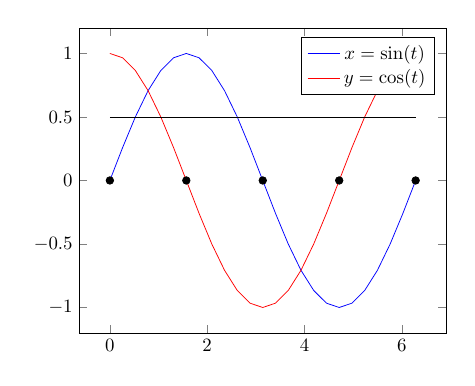
\begin{tikzpicture}[scale=0.68]%[scale=0.68]
    \begin{axis}[domain=0:2*pi,legend pos=north east]
    %\addplot[samples=12,mark=x,color=red] {sin(deg(x))}; 
    %\addplot[samples=12,mark=*,color=blue] {cos(deg(x))}; 
    \addplot[mark=none,color=blue] {sin(deg(x))}; 
    \addplot[mark=none,color=red] {cos(deg(x))}; 
    \addplot[mark=none,color=black]{0.5};
    %\addplot[mark=square,color=black] {0*deg(x)};
    \addplot[only marks,color=black] coordinates {
        (0,0)
        (0.5*pi,0)
        (pi,0)
        (1.5*pi,0)
        (2*pi,0)
    };
    \legend{$x=\sin(t)$,$y=\cos(t)$}
    \end{axis}
\end{tikzpicture}
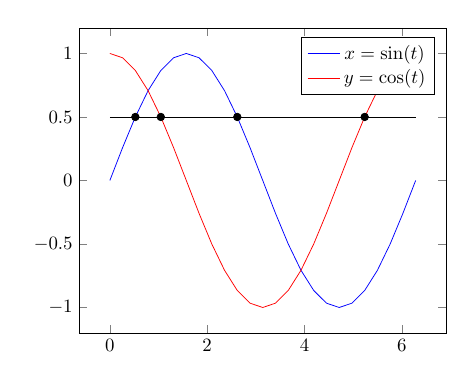
\begin{tikzpicture}[scale=0.68]
    \begin{axis}[domain=0:2*pi,legend pos=north east]
    \addplot[mark=none,color=blue] {sin(deg(x))}; 
    \addplot[mark=none,color=red] {cos(deg(x))}; 
    \addplot[mark=none,color=black]{0.5};
    \addplot[only marks,color=black] coordinates {
        (pi/6,0.5)
        (pi/3,0.5)
        (5*pi/6,0.5)
        (5*pi/3,0.5)
       % (0,0)
       % (0.5*pi,0)
       % (pi,0)
       % (1.5*pi,0)
       % (2*pi,0)
    };
    \legend{$x=\sin(t)$,$y=\cos(t)$}
    \end{axis}
\end{tikzpicture}

    \caption[Discretization]{Adapted version of discretization to asynchronous systems}
    \label{fig:discretization}
\end{figure}


This PhD thesis focuses on the study of reachability of asynchronous modeling frameworks.
We will still introduce in the last part of this section, a more global semantics.

\subsection{Generalized Semantics}
Generalized semantics is even more complex than asynchronous semantics.
Given a BN and a current state, if there are $m$ variables which may change their value at the next time point, there will be $2^m$ possibilities of the next state.

\begin{example}
Let us take the same transition interpretation table as Example~\ref{example:counterSynchronous}, we can update any number of variables at each time point.
The generalized case is shown in Figure~\ref{fig:updateScheme} (c).
\end{example}

To sum up, Table~\ref{tab:semantics} shows the difference of those three update schemes.

For synchronous update scheme, $m$ is the number of different variables in all the heads of rule.
The formal definition $m$ is as follows:
let $R$ be the set of rules and current state be $S=\init{var_0^{val_0},\cdots, var_n^{val_n}}$. 
$V=\{head(r)\mid \exists r\in R, body(r)\subseteq S\}$, then $m=|V|$.

For synchronous cases we can consider the possible future states is of $O(1)$ as it is little probable that many rules are in conflict even though one can create an extreme counterexample making the number of possible future states reach its theoretical limit $O(3^m)$ if the number of total states of all the variables is fixed (the proof is given in Appendix~\ref{sec:proof}).
The possible future states is polynomial for asynchronous cases.
However generalized update scheme has to consider the combinatorial results of the fireable transitions.

The benchmark part of~\cite{ribeiro2018learning} shows the complexity of generalized semantics, where the model inference fails with 12 components in the model. 

\begin{table}[ht]
    \centering
    \small
    \begin{tabular}{l|c|c|c}
        &Synchronous&Asynchronous&Generalized\\
        \hline
        nb of fireable transitions&\multicolumn{3}{c}{$n$}\\
        \hline
        nb of transitions \textit{will} be fired&$m$&$\min(1,m)$&$[0;m]$\\
        \hline
        nb of possible future states& at most $O(3^m)$&$m$&$[2^m;2^n]$
    \end{tabular}
    \caption[Update schemes]{Numbers of fireable transitions in different updating scheme, where $m$ stands for the number of different variables in all the heads of fireable rule.}
    \label{tab:semantics}
\end{table}

\section{Model Checking}\label{sec:modelchecking}
Model Checking is an automatic verification technique for large state transition systems and was independently developed by Clarke and Emerson~\cite{clarke1981design} and by Queille and Sifakis~\cite{queille1982specification} in the early 1980s. It was originally developed for reasoning about finite-state concurrent systems.
Typically, a model checker has three basic components: a modeling formalism adopted to encode a state machine representing the system to be verified, a specification language based on Temporal Logic, and a verification algorithm~\cite{clarke20142} which employs an exhaustive searching of the entire state space to determine whether the specification holds or not.

In this thesis we focus on reachability (\textbf{EF} in Temporal Logic) as most temporal properties can be reduced to reachability problems due to the expressiveness of hybrid modeling frameworks.

\subsection{Exact Model Checkers}
At first, Model Checking was done by the search in the state transition graphs, which are encoded in adjacent lists~\cite{clarke1981design}.
This representation however requires a memory growing exponentially with the number of components.
To avoid such explicit representation, state transition graphs were replaced by Boolean formulas.
OBDD (Ordinary Binary Decision Diagram) based Model Checkers were developed, having reached $10^{120}$ states, e.g.
SMV~\cite{mcmillan1993symbolic}, NuSMV~\cite{cimatti2000nusmv}, and VIS~\cite{brayton1996vis}.
However, the performance is still not enough to analyze problems in systems biology (time-memory out), which is illustrated in Chapter~\ref{chap:test}.  

\subsection{Static Analyzers}
Model Checkers are widely applied to hardware and software.
Especially when applied to software, algorithmic verification techniques have
to deal with software’s infinite state space, requiring abstraction techniques to make problems tractable.
SPIN~\cite{holzmann1997model} and Goanna~\cite{fehnker2006goanna} are designed as source code analyzers, by verifying a set of over-approximate conditions, they managed to check the safety/liveness properties of a program or whether certain program behaves as expected. 
However, the static code analyzers only determine run-time properties of programs by examining the code structure, which may produce false-positive and false-negative results~\cite{vorobyov2010comparing}.

Inspired by these ideas, Pint~\cite{Pint} takes the initiative to apply pure static analysis, combine over-approximation and under-approximation~\cite{pauleve2012} to squeeze the state space in order to try to solve the original reachability problem of a PH or an AAN (See Figure~\ref{fig:vennDiagram}).
Similarly, due to the approximations, the result of Pint is not necessarily conclusive~\cite{folschette2015}.

\begin{figure}[ht]
    \centering
    \begin{tikzpicture}[scale=0.8]
  \coordinate (c) at (0,0);
  \draw[thick,blue,rounded corners=1mm,dashed] (c) \irregularcircle{3cm}{3mm};
  %\draw[blue] (-1.2,-1.2) -- (1.2,-1.2) -- (1.2,1.2) -- (-1.2,1.2) -- (-1.2,-1.2);
  \draw[thick,purple] (-2.5,-1.2) -- (2.5,-1.2) -- (2.5,1.2) -- (-2.5,1.2) -- (-2.5,-1.2);
  \draw[thick,purple] (-7,-3.5) -- (3.5,-3.5) -- (3.5,3.5) -- (-7,3.5) -- (-7,-3.5);
  \node (under) at (0,0) {Under-approximation};
  \node [text width=3cm] (over) at (-4.8,0) {Over-\\approximation};
  \node (real) at (0,2) {Real dynamics};
\end{tikzpicture}
    \caption[Static analysis]{Schema of real dynamics and over-approximation and under-approximation in Pint}
    \label{fig:vennDiagram}
\end{figure}

\subsection{Reachability Problem}
In the domain of model checking, reachability has been of great interest for over 30 years~\cite{clarke2008birth,clarke20142}. 
Various modeling frameworks and semantics in bioinformatics have been studied: Boolean network~\cite{akutsu2007control}, Petri nets~\cite{mayr1984,esparza1998}, timed-automata~\cite{Daws1998,wozna2003}. 
These approaches rely on global search and thus face state explosion problem as the state space grows exponentially with the number of variables. 
In~\cite{peterson1977petri}, it has been shown that the reachability problem of Petri net is exponential time-hard and exponential space-hard, and this conclusion does not change even under some specific conditions~\cite{esparza1998}. 
For 1-safe Petri nets, the complexity of reachability analysis is generally PSPACE-complete~\cite{cheng1995complexity}.
Li \textit{et al.}~\cite{li2012reachability,li2014stability} investigated theoretically the stability, the controllability and the reachability of Switched Boolean Networks, but their method remains computationally expensive;
Saadatpour \textit{et al.}~\cite{saadatpour2010attractor} researched only the reachability of fixed points.

To tackle the complexity issue, symbolic model checking~\cite{burch1992symbolic} based on OBDDs and SAT-solvers (satisfiability)~\cite{abdulla2000symbolic} have been studied over years, but still fail to analyze big biological systems with more than $1000$ variables. 
Bounded Model Checking (BMC)~\cite{clarke2001bounded} is an efficient approach but generally not complete as its searching depth is limited to a given integer $k$.

Model checking is not only related to the verification of models, it can be of help to the learning of model and modification according to the unsatisfied properties.

\section{Model Learning and Model Revision}
All the modeling frameworks and model-checkers mentioned above are not effective unless they are fed with trustworthy system topology.
Model learning is used to classify the original data into generalized topological knowledge of the system where the original data come from raw data after being discretized, normalized, denoised \textit{etc.}
In this thesis we do not assess the quality of raw data as it is related to the results of biological experiments.

Among the important contributions, Khalis\textit{et al.}~\cite{khalis2009smbionet} have studied parameter learning in a given model topology.
Rodrigues \textit{et al.}~\cite{rodrigues2011active} have studied active learning of relational action model whose dynamics is however not compatible with BRNs.
Bonneau \textit{et al.}~\cite{bonneau2006inferelator} have developed a learning algorithm based on regression but with the limit on the size of clusters.
Opgen-Rhein \textit{et al.}~\cite{opgen2007correlation} have studied the learning using correlation coefficients, but their resulting regulatory networks are undirected. 
Ribeiro \textit{et al.} have designed LFIT-based (Learning From Interpretation Transitions) learning methods~\cite{ribeiro2015learning,ribeiro2018learning,ribeiro2017inductive} but these approaches cannot deal with noisy or imprecise inputs as all the errors are taken into account during the learning phase.

However, the sensitivity of LFIT can be of benefit in model revision.
The choices of revised models are often combinatorial w.r.t the satisfiability of certain dynamic properties.
If we consider another constraint that the revised model has to reproduce exactly the input time-series data, the number of consistent revised models will decrease.
Here we introduce some basic ideas of LFIT which will be of help in Chapter~\ref{chap:modelInference}.

As for model revision, to our knowledge, model revision based on reachability properties has never been considered in the literature.
One possible related work is cut set to be introduced after LFIT.
Cut set is used to detect the atoms cutting critical paths from the initial state and the desired states.
By inhibit these elements, we can ensure the unreachability of the desired states.
In practice, cut sets are useful for proposing potential therapeutic targets that have been formally identified from the model for preventing the activation of a particular molecule.
However, cut sets are not of direct help in model revision, as they inhibit certain atoms to be reached rather than modifying the system topology.

\subsection{Learning From Interpretation Transitions (LFIT)}\label{sec:lfitSyn}
LFIT aims at learning a logic program $P$ (definition in Section~\ref{sec:logicProgram} on page \pageref{sec:logicProgram}) from a set of state transitions $E$ in the form $S_1\to S_2$ where $S_1,S_2$ are the states of the system.
$E$ can be extracted from discretized time-series data.
Here LFIT considers only synchronous updating scheme, hence we name it as ``synchronous LFIT''.

Basically, the mechanics of synchronous LFIT is as follows: it starts from the most general logic program.
It verifies whether every element in $E$ is consistent with $P$.
Obtained inconsistencies are classified as conflicts.
Then LFIT tries to specialize the conflicting rules by adding atoms in their body to make them harder to be matched.
When there is no conflict, $P$ can reproduce perfectly all the state transitions in $E$.

Algorithm~\ref{alg:syncLFIT} in Appendix~\ref{chap:algo} describes the details of synchronous LFIT.
To prevent potential ambiguities, we denote assignment operation as $:=$ instead of $\gets$. 


\subsection{Cut set}\label{sec:cutset}

Paulev\'e \textit{et al.}~\cite{PAK13-CAV} have designed an algorithm for identifying sets of atoms whose activity is necessary for the reachability of a given local state. 
If all the atoms from such a set are disabled in the model, the concerned reachability is impossible. 
Those sets are referred to as cut sets and are computed from a particular abstract causality structure, so-called Local Causality Graph (detailed in Section~\ref{sec:SLCG}).
\textit{Via} such manipulation on atoms, one may control certain dynamical properties of a BRN.

However, we are going to try to control the systems dynamics by revising the transition rules of a model instead of inhibiting/imposing certain atoms.
This need urges us to make modifications on the elements to be inhibited.
The detail of cut sets is in Section~\ref{sec:cutsetModelInfer}. 

\section{R\'esum\'e}
In this chapter, we presented mainly four main basic contents of the state of the art:

\begin{itemize}
    \item Modeling frameworks
    \item Update schemes of models
    \item Model checking and model checkers
    \item Model learning/inference techniques
\end{itemize}

Modeling frameworks allow one to encode real biological regulatory systems into computable models according to his need (completion, static analysis, dynamic analysis, simulation \textit{etc.}).
In the next chapter, we will focus on a finer reachability analysis.
To achieve this goal, we will propose a new modeling framework ABAN based on existing ones presented in this chapter.
Also, to better position our new modeling framework and define its dynamics, we introduced different update schemes of models.
To validate and evaluate our work (in Chapter~\ref{chap:test}), we introduced here several representative model checkers to be used for comparison.
With the help of model learning technique LFIT and our reachability analysis methods, we managed to develop a model revision method based on desired reachability properties which has never been consider before.